\chapter{Resultados}

\subsection{Prueba académica}

Las 15 personas que hicieron la prueba tuvieron ambas respuestas correctas, identificando correctamente el recorrido BFS y DFS en cada caso.


\subsection{Formulario MEEGA+: Percepción de usuario}

% Hablar de la suma de puntaje y puntaje promedio para los dos casos: De fase exploratoria y fase posterior.
% Poner acá gráficos y demás
Según \cite{meegaplus} un set de respuestas de un individuo se considera correcto y válido cuando tiene más del 85\% de las preguntas contestadas. En este caso no hubo omisiones.

En la figura \ref{RespuestasAgregadas} se muestran los resultados agregados para cada pregunta en cada categoría. Las preguntas se acortaron con acrónimos, pero la indexación está disponible en el anexo: 

\begin{figure}[h]
	\centering
	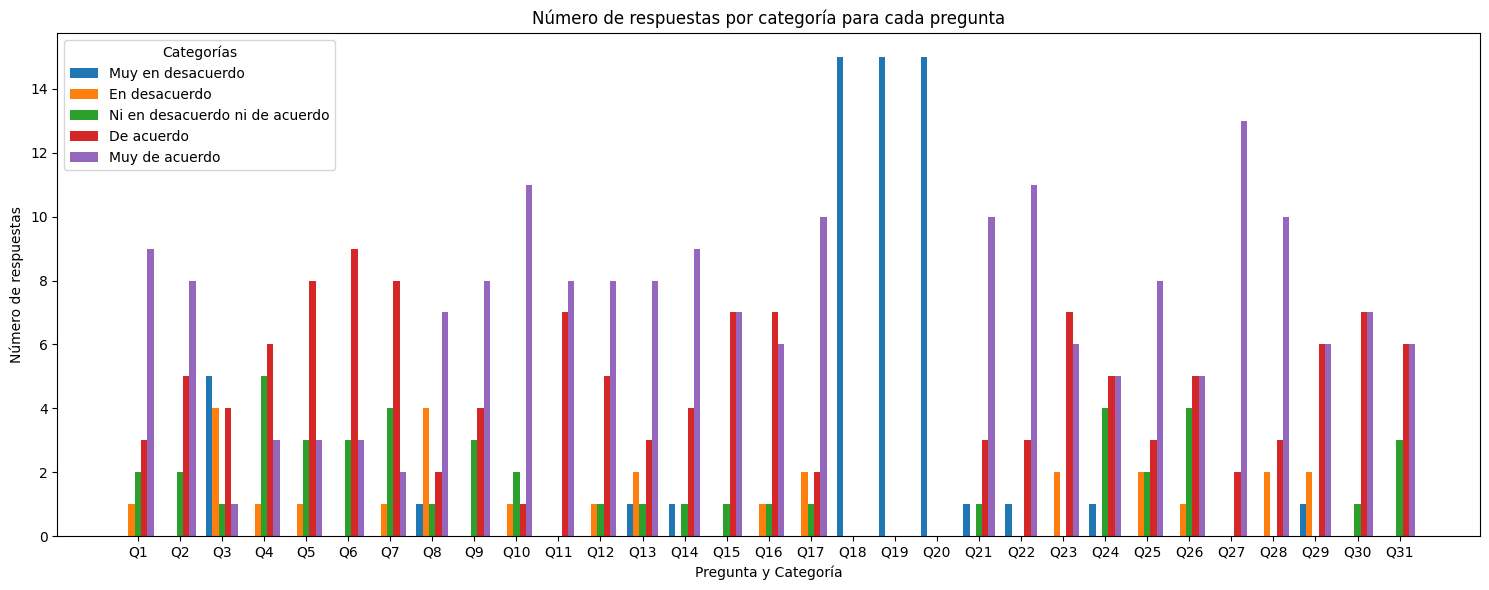
\includegraphics[scale=.5]{imagenes/answers.png}
	\caption{Agregación de respuestas por categoría y por pregunta}
	\label{RespuestasAgregadas}
\end{figure}

